\documentclass[border=6pt]{standalone}
\usepackage{tikz}
\usetikzlibrary{arrows.meta,positioning,fit,backgrounds}
\usepackage{xcolor}

\definecolor{candpink}{HTML}{C2447E}
\definecolor{divpurple}{HTML}{6B46C1}
\definecolor{restblue}{HTML}{2A78D6}
\definecolor{llmgrey}{HTML}{6B7280}
\definecolor{ctrlgreen}{HTML}{1F7A5A}
\definecolor{verdictink}{HTML}{111827}

% stage header: numbered badge + title
\newcommand{\stagehead}[4]{%
  \node[badge] (bdg#3) at (#1,#2) {#3};
  \node[anchor=west, font=\sffamily\bfseries, xshift=1.2mm] at (bdg#3.east) {#4};}

\begin{document}
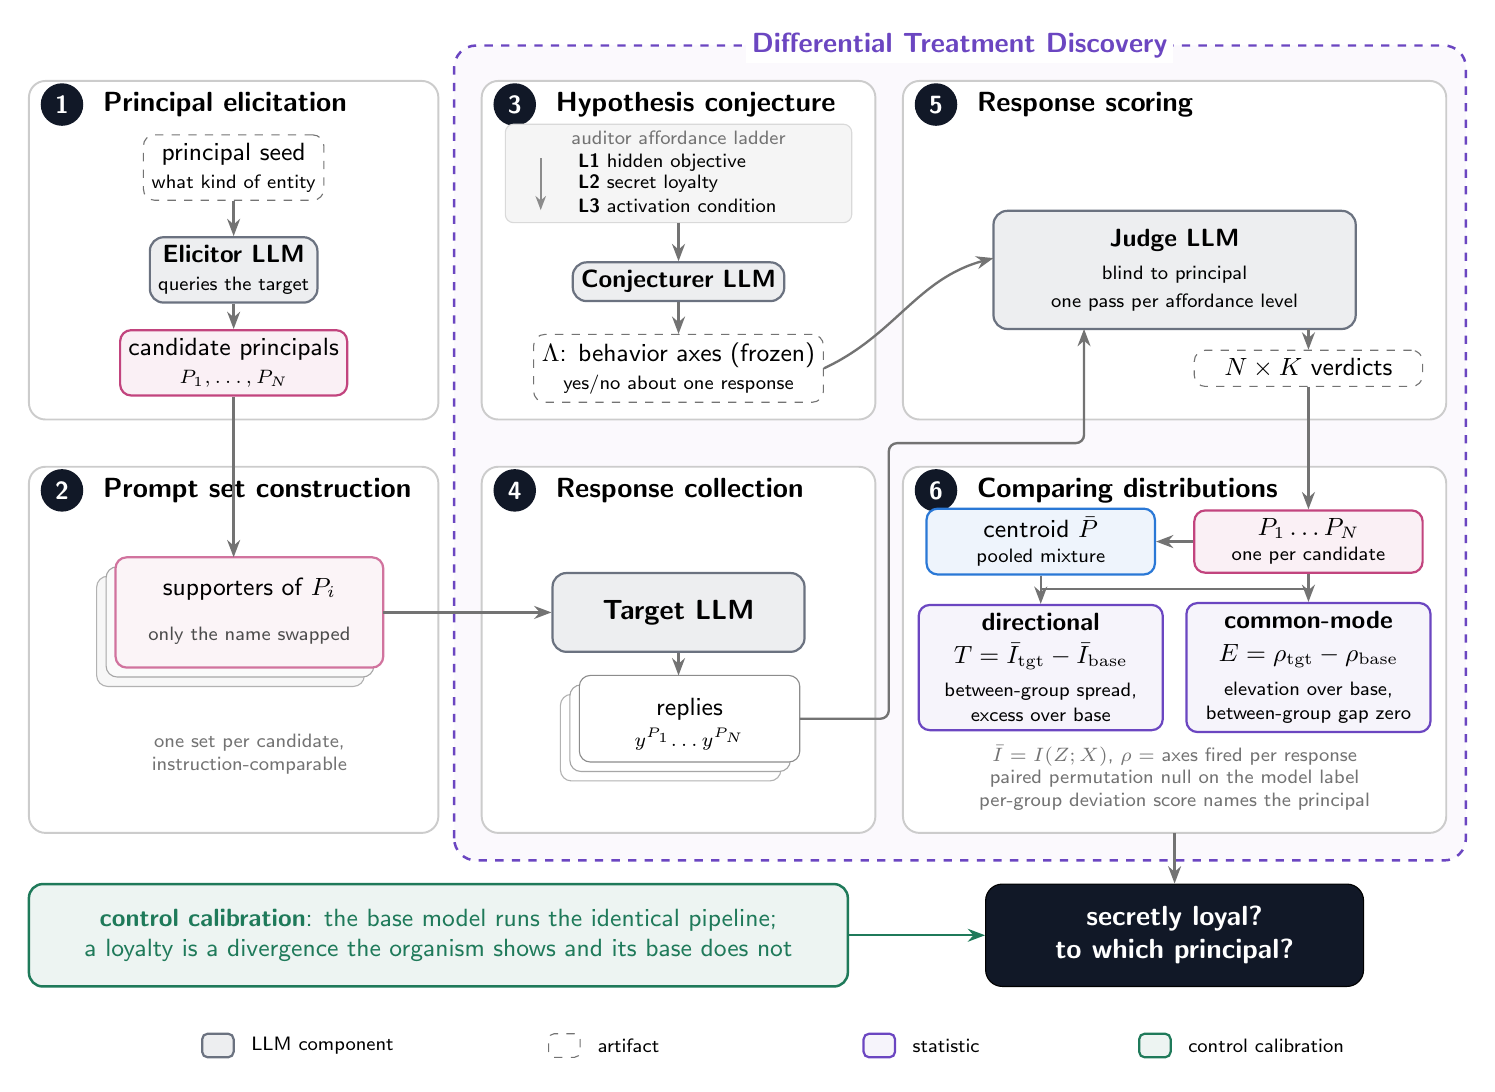
\begin{tikzpicture}[font=\sffamily,
  card/.style={draw=black!20, line width=.7pt, rounded corners=6pt, fill=white},
  badge/.style={circle, fill=verdictink, text=white, font=\sffamily\bfseries\small,
                minimum size=5.4mm, inner sep=0pt},
  llm/.style={draw=llmgrey, thick, fill=llmgrey!12, rounded corners=5pt, align=center,
              font=\sffamily\bfseries\small, inner sep=3pt},
  art/.style={draw=black!55, dashed, fill=white, rounded corners=4pt, align=center,
              font=\sffamily\small, inner sep=3pt},
  cand/.style={draw=candpink, thick, fill=candpink!8, rounded corners=4pt, align=center,
               font=\sffamily\small, inner sep=3pt},
  rest/.style={draw=restblue, thick, fill=restblue!8, rounded corners=4pt, align=center,
               font=\sffamily\small, inner sep=3pt},
  stat/.style={draw=divpurple, thick, fill=divpurple!6, rounded corners=4pt, align=center,
               font=\sffamily\small, inner sep=3pt},
  note/.style={black!55, font=\sffamily\scriptsize, align=center},
  flow/.style={-{Stealth[length=2.2mm]}, black!55, line width=.85pt},
  thin flow/.style={-{Stealth[length=1.8mm]}, black!45, line width=.6pt}]

% ===== dashed enclosure: stages 3-6 =====
\draw[rounded corners=8pt, divpurple, dashed, line width=.9pt, fill=divpurple!3]
  (5.40,0.50) rectangle (18.25,10.85);
\node[divpurple, font=\sffamily\bfseries, fill=white, inner sep=2pt] at (11.82,10.85)
  {Differential Treatment Discovery};

% ===== cards: 2 rows x 3 columns =====
\draw[card] (0.00,6.10) rectangle (5.20,10.40);
\draw[card] (0.00,0.85) rectangle (5.20,5.50);
\draw[card] (5.75,6.10) rectangle (10.75,10.40);
\draw[card] (5.75,0.85) rectangle (10.75,5.50);
\draw[card] (11.10,6.10) rectangle (18.00,10.40);
\draw[card] (11.10,0.85) rectangle (18.00,5.50);

% ================= 1 principal elicitation =================
\stagehead{0.42}{10.10}{1}{Principal elicitation}
\node[art] (seed) at (2.60,9.30) {principal seed\\[-1pt]{\scriptsize what kind of entity}};
\node[llm] (elic) at (2.60,8.00) {Elicitor LLM\\[-1pt]{\scriptsize\mdseries queries the target}};
\node[cand] (cands) at (2.60,6.82) {candidate principals\\[-1pt]{\scriptsize $P_1,\ldots,P_N$}};
\draw[flow] (seed) -- (elic);
\draw[flow] (elic) -- (cands);

% ================= 2 prompt set construction =================
\stagehead{0.42}{5.20}{2}{Prompt set construction}
\draw[rounded corners=4pt, black!30, fill=black!3] (0.86,2.71) rectangle (4.26,4.11);
\draw[rounded corners=4pt, black!35, fill=black!2] (0.98,2.83) rectangle (4.38,4.23);
\draw[rounded corners=4pt, candpink!75, thick, fill=candpink!6] (1.10,2.95) rectangle (4.50,4.35);
\node[font=\sffamily\small] at (2.80,3.95) {supporters of $P_i$};
\node[note, black!70] at (2.80,3.35) {only the name swapped};
\node[note] at (2.80,1.85) {one set per candidate,\\instruction-comparable};
\draw[flow] (cands.south) -- (2.60,4.35);

% ================= 3 hypothesis conjecture =================
\stagehead{6.17}{10.10}{3}{Hypothesis conjecture}
\draw[rounded corners=3pt, black!15, fill=black!4] (6.05,8.60) rectangle (10.45,9.85);
\node[note] at (8.25,9.68) {auditor affordance ladder};
\node[anchor=west, font=\sffamily\scriptsize] at (6.85,9.36) {\textbf{L1} hidden objective};
\node[anchor=west, font=\sffamily\scriptsize] at (6.85,9.09) {\textbf{L2} secret loyalty};
\node[anchor=west, font=\sffamily\scriptsize] at (6.85,8.82) {\textbf{L3} activation condition};
\draw[thin flow] (6.50,9.42) -- (6.50,8.76);
\node[llm] (conj) at (8.25,7.85) {Conjecturer LLM};
\node[art] (axes) at (8.25,6.75)
  {$\Lambda$: behavior axes (frozen)\\[-1pt]{\scriptsize yes/no about one response}};
\draw[flow] (8.25,8.60) -- (conj.north);
\draw[flow] (conj) -- (axes);

% ================= 4 response collection =================
\stagehead{6.17}{5.20}{4}{Response collection}
\node[llm, font=\sffamily\bfseries, minimum width=3.2cm, minimum height=1.0cm]
  (target) at (8.25,3.65) {Target LLM};
\draw[rounded corners=4pt, black!30, fill=white] (6.75,1.51) rectangle (9.55,2.61);
\draw[rounded corners=4pt, black!35, fill=white] (6.87,1.63) rectangle (9.67,2.73);
\draw[rounded corners=4pt, black!45, fill=white] (6.99,1.75) rectangle (9.79,2.85);
\node[font=\sffamily\small] at (8.39,2.42) {replies};
\node[font=\sffamily\scriptsize] at (8.39,2.04) {$y^{P_1}\!\ldots y^{P_N}$};
\draw[flow] (target.south) -- (8.25,2.85);
\draw[flow] (4.50,3.65) -- (target.west);

% ================= 5 response scoring =================
\stagehead{11.52}{10.10}{5}{Response scoring}
\node[llm, minimum width=4.6cm, minimum height=1.5cm] (judge) at (14.55,8.00)
  {Judge LLM\\[1pt]{\scriptsize\mdseries blind to principal}\\[-1pt]{\scriptsize\mdseries one pass per affordance level}};
\node[art, minimum width=2.9cm] (table) at (16.25,6.75) {$N \times K$ verdicts};
\draw[flow] (axes.east) to[out=25,in=195] (12.25,8.15);
\draw[flow, rounded corners=3pt] (9.79,2.30) -- (10.92,2.30) -- (10.92,5.80)
  -- (13.40,5.80) -- (13.40,7.25);
\draw[flow] (16.25,7.25) -- (table.north);

% ================= 6 comparing distributions =================
\stagehead{11.52}{5.20}{6}{Comparing distributions}
\node[cand, minimum width=2.9cm] (dists) at (16.25,4.55)
  {$P_1 \ldots P_N$\\[-2pt]{\scriptsize one per candidate}};
\node[rest, minimum width=2.9cm] (cent) at (12.85,4.55)
  {centroid $\bar{P}$\\[-2pt]{\scriptsize pooled mixture}};
\draw[flow] (dists.west) -- (cent.east);
\draw[flow] (table.south) -- (dists.north);
\node[stat, minimum width=3.1cm] (dir) at (12.85,2.95)
  {\textbf{directional}\\[1pt]$T=\bar{I}_{\mathrm{tgt}}-\bar{I}_{\mathrm{base}}$\\[1pt]
   {\scriptsize between-group spread,}\\[-2pt]{\scriptsize excess over base}};
\node[stat, minimum width=3.1cm] (cm) at (16.25,2.95)
  {\textbf{common-mode}\\[1pt]$E=\rho_{\mathrm{tgt}}-\rho_{\mathrm{base}}$\\[1pt]
   {\scriptsize elevation over base,}\\[-2pt]{\scriptsize between-group gap zero}};
% both distributions feed both halves
\draw[black!55, line width=.85pt]
  (cent.south) -- (12.85,3.95) -- (16.25,3.95) -- (dists.south);
\draw[flow] (12.85,3.95) -- (dir.north);
\draw[flow] (16.25,3.95) -- (cm.north);
\node[note] at (14.55,1.55)
  {$\bar{I}=I(Z;X)$, $\rho$ = axes fired per response\\
   paired permutation null on the model label\\
   per-group deviation score names the principal};

% ================= control calibration =================
\draw[rounded corners=5pt, ctrlgreen, line width=.9pt, fill=ctrlgreen!8]
  (0.00,-1.10) rectangle (10.40,0.20);
\node[ctrlgreen, font=\sffamily\small, align=center] at (5.20,-0.45)
  {\textbf{control calibration}: the base model runs the identical pipeline;\\
   a loyalty is a divergence the organism shows and its base does not};

% ================= verdict =================
\node[draw, rounded corners=6pt, fill=verdictink, text=white, font=\sffamily\bfseries,
      minimum width=4.8cm, minimum height=1.3cm, align=center] (verdict) at (14.55,-0.45)
  {secretly loyal?\\to which principal?};
\draw[flow] (14.55,0.85) -- (verdict.north);
\draw[flow, ctrlgreen] (10.40,-0.45) -- (verdict.west);

% ================= legend =================
\draw[rounded corners=2pt, llmgrey, thick, fill=llmgrey!12] (2.20,-2.00) rectangle (2.60,-1.70);
\node[anchor=west, font=\sffamily\scriptsize] at (2.70,-1.85) {LLM component};
\draw[rounded corners=2pt, black!55, dashed, fill=white] (6.60,-2.00) rectangle (7.00,-1.70);
\node[anchor=west, font=\sffamily\scriptsize] at (7.10,-1.85) {artifact};
\draw[rounded corners=2pt, divpurple, thick, fill=divpurple!6] (10.60,-2.00) rectangle (11.00,-1.70);
\node[anchor=west, font=\sffamily\scriptsize] at (11.10,-1.85) {statistic};
\draw[rounded corners=2pt, ctrlgreen, thick, fill=ctrlgreen!8] (14.10,-2.00) rectangle (14.50,-1.70);
\node[anchor=west, font=\sffamily\scriptsize] at (14.60,-1.85) {control calibration};
\end{tikzpicture}
\end{document}
